\scanpage{130}
% archive foliation: 129
hémisphères par un équateur, avec $1$ ou
deux sommets dessus (donc suivant les
cas, $1$ sommet et une arête, ou $2$ sommets
et $2$ arêtes) le groupe des automorphismes
holomorphes qui fixe la carte et ses
él. de structure (donc induit un
autom. isotope à $1$) est le groupe des
$z\mapsto\dfrac{az\unsure{-|+}b}{cz+d}$ ($a,b,c,d\in\mathbb{R}$, $ad-bc=1$) qui fixe
$\infty$ (donc $c=0$ \inserted{on trouve le groupe $\operatorname{Aff}(1,\unsure{\mathbb{C}|\mathbb{R}})$} \deleted{de Lie $2$})
soit $0$ et $\infty$ (groupe $\unsure{\mathbb{C}^*|\mathbb{R}^*}$ de dim $1$).

Autre exemple:
\figure{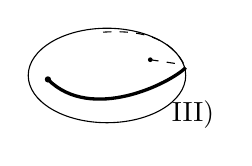
\begin{tikzpicture}[x=1cm,y=1cm]
\draw(0,0)ellipse(1 and .6);\draw[line width=1.2pt](-.75,-.05)..controls(-.2,-.6)and(.8,-.1)..(1,.1);\draw[dashed](-.05,.55)..controls(.7,.6)and(.9,.3)..(1,.1);\fill(-.75,-.05)circle(.04);\fill(.55,.2)circle(.03);\draw[dashed](.55,.2)--(.95,.14);\node[right]at(.7,-.5){III)};
\end{tikzpicture}}
($1$ arête, $2$ sommets,
duale de $1$ arête $1$ sommet) qui a
le même groupe $\operatorname{Aff}(1,\mathbb{C})$. // Si on exige
que \deleted{\unsure{les bords des}} \inserted{chaque \deleted{\unsure{face}} comp. de $X$ ait une}
face \inserted{dont l'ordre} soit au
moins trois, a-t-on gagné? J'ai
l'impression que oui, grâce à la
théorie de la représentation conforme.
\margin{au moins pour les cartes finies\ldots}
La condition envisagée signifie que
Les composantes connexes sont \unsure{toutes}
distinctes de la sphère munie
soit de la carte de type $(2,1)$ (cas I)
